\documentclass[12pt]{exam}
\RequirePackage{amssymb, amsfonts, amsmath, latexsym, verbatim, xspace, setspace, mathpazo, multicol, xcolor}


% Multicols
\usepackage{multicol}

% Color
\usepackage{xcolor}


% Font
\usepackage{anyfontsize}
%\usepackage[default,regular,black]{sourceserifpro}
%\usepackage{tgpagella,eulervm}
\usepackage[T1]{fontenc}

\usepackage{tabto}

\usepackage{ifthen}
\usepackage{mathtools}

\usepackage{pgfplots}

\makeatletter
\newenvironment{noparchoices}%
  {%
    \setcounter{choice}{0}%
    \def\choice{%
      \refstepcounter{choice}%
      \choicelabel\ 
      % No need to put the following into a token string; we just put
      % the choicelabel onto the page, so we're at the spot whose page
      % number we want to record:
      \questionobject@pluspagecheck
    }% choice
    \def\CorrectChoice{%
      \refstepcounter{choice}%
      \choicelabel\
      % No need to put the following into a token string; we just put
      % the choicelabel onto the page, so we're at the spot whose page
      % number we want to record:
      \questionobject@pluspagecheck
      \ifprintanswers
      \CorrectChoice@Emphasis
        \fi
    }% CorrectChoice
    \let\correctchoice\CorrectChoice
    % If we're continuing the paragraph containing the question,
    % then leave a bit of space before the first choice:
    \ignorespaces
  }%
\makeatother


\usepackage{geometry}
\geometry{left=0.38in,right=0.38in,%
bindingoffset=0mm, top=1em,bottom=4em}
\usepackage[none]{hyphenat}


\newcommand{\ibmatrix}[1]{\begin{bmatrix}#1\end{bmatrix}} % inline bmatrix

\newcommand{\separator}{\noindent{\rule[1ex]{0.45\textwidth}{.1pt}}}
\newcommand{\newquestion}[1]{
    {\fontsize{12}{14}\selectfont
    \uplevel{\separator \\[-2mm] [Qu.]
    \fontsize{14}{16}\selectfont
    \ifthenelse{\equal{#1}{}}{\ \\[-7mm]}{#1\\[-1em]}}
    }}
\renewcommand{\choicelabel}{(\alph{choice})}

\newcommand{\model}{MODEL 3}
\newcommand{\examnum}{Final Exam SSP EMPx19}
\newcommand{\examdate}{Spring 2025}


\renewcommand{\questionshook}{
    \setlength{\leftmargin}{2em}
    \setlength{\linewidth}{.45\textwidth}
}
\renewcommand{\questionlabel}{{\fontsize{12}{14}\selectfont\thequestion.}}
\renewcommand{\choicelabel}{(\alph{choice})}

\newcommand{\nextcol}{\vfill\mbox{}\columnbreak}

% \input{scheme.tex}

\newcommand{\barchart}[1]{
\hspace{-8pt}\begin{tikzpicture}[scale=0.40]
        \begin{axis}[
            ybar,xlabel={},ylabel={Frequency},ylabel style={font=\bfseries, yshift=-20pt},ymin=0,xmin=0,xtick={2,4,6,8,10},xticklabels={2,4,6,8,10},visualization depends on={y\as\YY},nodes near coords={\pgfmathtruncatemacro{\YY}{ifthenelse(\YY==0,0,1)}\ifnum\YY=0\else\pgfmathprintnumber\pgfplotspointmeta\fi},nodes near coords style = {anchor=south west,text width=8mm, inner xsep=4pt, align=center},bar width=15pt,axis lines*=left,y axis line style={->,very thick},x axis line style={->, very thick},yticklabel style={draw=none},ytick=\empty]
            \addplot[ybar interval] coordinates {#1};
            \end{axis}
        \end{tikzpicture}    
}

\usepackage{leftindex}

\newcommand{\comb}[2]{\leftindex^{#1}{\text{C}}_{#2}}


\usepgfplotslibrary{statistics}

\begin{document}


\footrule
\firstpagefooter{\model ~~~~~~~~ \examnum~ \examdate}{}{Page \thepage~of \numpages}
\runningfooter{\model ~~~~~~~~ \examnum~ \examdate}{}{Page \thepage~of \numpages}

\setlength{\columnseprule}{.1pt}
\def\columnseprulecolor{\color{black}}

\pointformat{}
\pointsinmargin

\begin{multicols*}{2}
	\noindent
	\textbf{\examnum~\examdate} \\[-8mm]
	\begin{questions}
		\fontsize{14}{16}\selectfont
		\addpoints
		\begingradingrange{exam}
		\newquestion{Consider the following sample: \linebreak $\lbrace 0.1, 0.2, \text{\textbf{\underline{A}}}, 0.3, 0.3, 2.1, 2.1, 2.1, 5.8, \text{\textbf{\underline{B}}}, 10, 10 \rbrace$.\linebreak The sample values are sorted in \textbf{\underline{ascending}} order. It is given that the third quartile $Q_3 = 5.85$ and sample modes=0.3 and 2.1.}

		\question[1] The unknown entries of the sample, $\text{\textbf{A}} = \dots$ and $\text{\textbf{B}} = \dots$

		\begin{noparchoices}
			\begin{tabular}{cccc}
				\choice & $0.2, 5.8$ & \choice & $0.25, 5.85$ \\
				\choice & $0.3, 5.9$ & \choice & $0.3, 5.85$  \\
				\choice & $0.3, 10$  & \choice & $0.2, 5.9$   \\
			\end{tabular}
		\end{noparchoices}

		\question[1] The sample mean $\overline{x} = \dots$ and \linebreak median $\tilde{x} = \dots$

		\begin{noparchoices}
			\begin{tabular}{clcc}
				\choice & $3.2, 5.8$   & \choice & $3.267, 2.1$ \\
				\choice & $3.262, 2.1$ & \choice & $3.2, 1.2$   \\
				\choice & $3, 1.2$     & \choice & $3, 3.95$    \\
			\end{tabular}
		\end{noparchoices}

		\question[1] Using 5 bins and a range from 0 to 10, the histogram will be

		\begin{noparchoices}
			\begin{tabular}{llll}
				\choice & \barchart{(0, 3) (2, 5) (4, 2) (6,0) (8, 2) (10, 0)} & \choice & \barchart{(0, 4) (2, 3) (4, 2) (6,2) (8, 2) (10, 0)} \\
				\choice & \barchart{(0, 2) (2, 2) (4, 3) (6,5) (8, 0) (10, 0)} & \choice & none                                                 \\
			\end{tabular}
		\end{noparchoices}

		\question[1] The box and whisker plot of the given sample will be
        
        \begin{oneparchoices}
            \choice 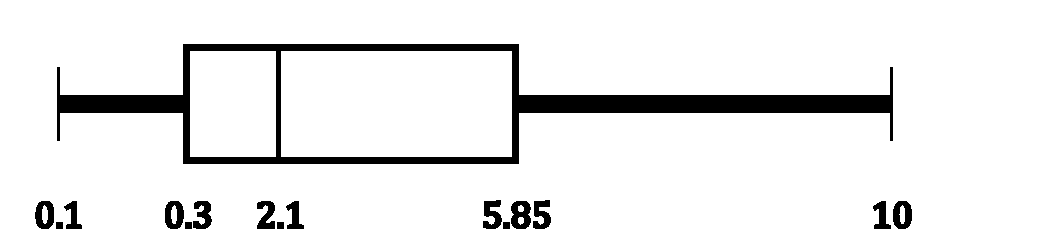
\includegraphics[scale=0.37]{a.pdf}
            \choice 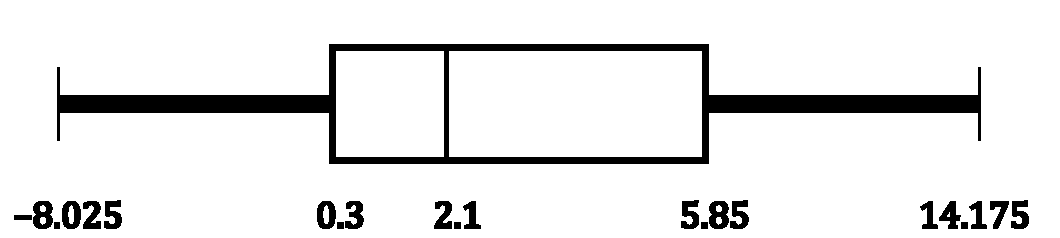
\includegraphics[scale=0.37]{b.pdf}
            \choice 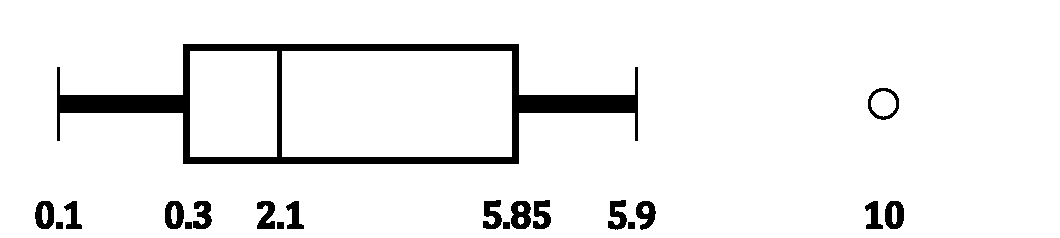
\includegraphics[scale=0.37]{c.pdf}
            \choice 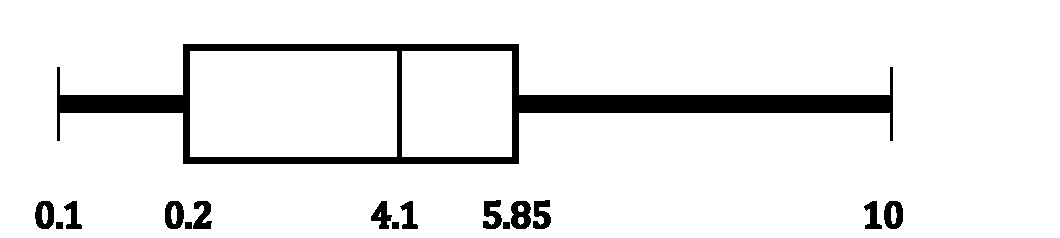
\includegraphics[scale=0.37]{d.pdf}
        \end{oneparchoices}

        \nextcol

        \question[1] Using the histogram and box plot, we suggest a .... PDF

        \begin{oneparchoices}
            \choice left ($-$) skewed\\
            \choice right ($+$) skewed\\
            \choice symmetric\\
            \choice uniform
        \end{oneparchoices}

        \question[1] If the sample has outliers, which measure of central tendency is not affected at all by outliers?

		\begin{noparchoices}
			\begin{tabular}{lllc}
				\choice & sample variance & \choice & median \\
				\choice & $Q_1$           & \choice & $\overline{x}$ \\
                \choice & a and d         & \choice & mode \\
			\end{tabular}
		\end{noparchoices}

        \newquestion{Suppose that $\hat{\Theta}_1$ and $\hat{\Theta}_2$ are \linebreak estimators of the parameter $\theta$. We \linebreak know that $E(\hat{\Theta}_1) = \theta,~E(\hat{\Theta}_2) = \theta/2,\linebreak Var(\hat{\Theta}_1) = 10$ and $Var(\hat{\Theta}_2) = 4$. }

        \question[1] $E(\hat{\Theta}_1 - \theta)^2 = ..., E(\hat{\Theta}_2 - \theta)^2 = ...$

        \begin{noparchoices}
			\begin{tabular}{lllc}
				\choice & $10,\quad 4 + \frac{\theta^2}{4}$ & \choice & $10,\quad 4$ \\
				\choice & $ 0,\quad \frac{\theta}{2}      $ & \choice & $10,\quad 4 + \frac{\theta^2}{2}$ \\
                \choice & $10,\quad \frac{\theta^2}{4}    $ & \choice & $\theta + 10,\quad 4 + \frac{\theta^2}{4} $ \\
			\end{tabular}
		\end{noparchoices}

        \question[1] The biased estimator may be more efficient under the condition that

        \begin{noparchoices}
			\begin{tabular}{llll}
				\choice & $\theta^2 > 24$ & \choice & $n \rightarrow \infty$ \\
				\choice & $\theta < 12$   & \choice & $\theta^2 < 24$ \\
                \choice & $\theta > 12$   & \choice & $n \rightarrow 0$ \\
			\end{tabular}
		\end{noparchoices}

        \newquestion{Let $X_1, X_2, \dotsb, X_n, (n>1)$ be an independent and random sample taken \linebreak from a population having mean $\mu = 3\beta$\linebreak and variance $\sigma^2 = 3\beta^2$. Suppose that \linebreak $\hat{\beta}_1 = \frac{\overline{X}}{3}, \hat{\beta}_2 = \frac{X_1}{3}$ and $\hat{\beta}_3 = \frac{2X_1 - X_n}{3}$ are \linebreak three estimators of the parameter $\beta$.}
        \question[1] Which estimator(s) is/are\linebreak unbiased?

        \begin{noparchoices}
			\begin{tabular}{lllc}
				\choice & $\hat{\beta}_1$ only                  & \choice & $\hat{\beta}_1, \hat{\beta}_2, \hat{\beta}_3$ \\
				\choice & $\hat{\beta}_1, \hat{\beta}_2$ only   & \choice & $\hat{\beta}_1, \hat{\beta}_3$ only \\
                \choice & $\hat{\beta}_3$                       & \choice & none \\
			\end{tabular}
		\end{noparchoices}
        
        \nextcol

        \question[1] $MSE(\hat{\beta}_1) = ...~, MSE(\hat{\beta}_2) = ...~, \linebreak MSE(\hat{\beta}_3) = ... ~~^\textit{\footnotesize a}$

        \begin{noparchoices}
        	\begin{tabular}{lllc}
        		\choice & $\frac{\beta^2}{n}, \beta^2, \beta^2$ & \choice & $\frac{\beta^2}{n}, \beta^2, 5\beta^2$ \\
        		\choice & $\beta^2, \frac{\beta^2}{3}, \frac{\beta^2}{9}$   & \choice & $\beta^2, \frac{\beta^2}{3}, \frac{5\beta^2}{3}$\\
                \choice & $\frac{\beta^2}{3n}, \frac{\beta^2}{3}, \frac{5\beta^2}{3}$                       & \choice & none \\
        	\end{tabular}
        \end{noparchoices}
        
        \rule{3cm}{0.6pt}\\[-0.9cm]

        {\footnotesize ~~~~~ $^\textit{a}$MSE: Mean Square Error}
        
        \question[1] The most efficient estimator is ..., while the worst is ...

        \begin{noparchoices}
        	\begin{tabular}{lllc}
        		\choice & $\hat{\beta}_1,\quad \hat{\beta}_2$                                           & \choice & $\hat{\beta}_1,   \quad \hat{\beta}_3$ \\
        		\choice & $\hat{\beta}_2,\quad \hat{\beta}_3$                            & \choice & $\hat{\beta}_2,  \quad \hat{\beta}_1$ \\
                \choice & $\hat{\beta}_1,\quad (\hat{\beta}_2 \text{~and~} \hat{\beta}_3)$ & \choice & $\hat{\beta}_3,\quad  \hat{\beta}_2$ \\
        	\end{tabular}
        \end{noparchoices}

        \question[1] By checking the consistency of estimators, which estimator(s)\linebreak is/are consistent?

        \begin{noparchoices}
        	\begin{tabular}{lllc}
        		\choice & $\hat{\beta}_1$                               & \choice & $\hat{\beta}_1, \hat{\beta}_2$ \\
        		\choice & $\hat{\beta}_2, \hat{\beta}_3$                & \choice & $\hat{\beta}_2$ \\
                \choice & $\hat{\beta}_1, \hat{\beta}_2, \hat{\beta}_3$ & \choice & $\hat{\beta}_1, \hat{\beta}_3$ \\
        	\end{tabular}
        \end{noparchoices}

        \newquestion{Consider a normally distributed population $X$ with mean $\mu$ and a known\linebreak standard deviation $\sigma = 16$. An independent and random sample of size $n = 16$ gives a sample mean $\overline{X} = 10$.}

        \question[1] The distribution of \underline{$\overline{X}$} is Normal with standard deviation=...

        \begin{noparchoices}
            \begin{tabular}{lclc}
                \choice & 2 & \choice & 4 \\
                \choice & 6 & \choice & 16 \\
                \choice & 64 & \choice & none \\
            \end{tabular}
        \end{noparchoices}
        
        \question[1] We are $90\%$ confident that $\mu$ is \linebreak located within the interval...\\
        $(\Phi(1.96) = 0.975, \Phi(1.645) = 0.95,\linebreak \Phi(2.575) = 0.995)$

        \begin{noparchoices}
            \begin{tabular}{ll}
                \choice & $\lbrack 6.71 , 13.29 \rbrack$\\
                \choice & $\lbrack 2.16 , 17.84 \rbrack$\\
                \choice & $\lbrack -16.32 , 36.32 \rbrack$\\
                \choice & $\lbrack 3.42 , 16.58 \rbrack$\\
                \choice & $\lbrack -0.3 , 20.3 \rbrack$\\
            \end{tabular}
        \end{noparchoices}

        \nextcol

        \question[1] If it is required to minimize the maximum absolute error in estimating $\mu$ to be not more than 2 with the same confidence level (90\%), the smallest sample size that should be taken is

        \begin{noparchoices}
            \begin{tabular}{llll}
                \choice & 174 & \choice & 246 \\
                \choice & 425 & \choice & 100 \\
                \choice & 20  & \choice & 152 \\[-4mm]
            \end{tabular}
        \end{noparchoices}

        \newquestion{\fontsize{12}{14}Consider the population defined by\linebreak random variable $X$, whose moment generating function is $M_X(t)  = (1 - \beta t)^{-a}$. Let $X_1, X_2, \dotsm, X_n$ be an independent and random sample, resulting in $\overline{X} = 2$ and $\frac{1}{n} \sum_{i=1}^{n} x^2_i = 10$.\\[-9mm]}

        \question[1] $E(X) = ....$\\
        \begin{noparchoices}
            \begin{tabular}{lllc}
                \choice & $\frac{1}{\beta(\alpha - 1)}$ & \choice & $-\alpha$ \\
                \choice & $\alpha\beta$ & \choice &  $\frac{1}{(1-\alpha)}$ \\
                \choice & $-\alpha\beta$ & \choice & $-\alpha\beta(1-\beta t)^{-\alpha}$ \\[-4mm]
            \end{tabular}
        \end{noparchoices}

        \question[1] $E(X^2)=....$\\
        \begin{noparchoices}
            \begin{tabular}{lllc}
                \choice & $\alpha(\alpha-1)\beta^2$ & \choice & $-\alpha(\alpha+1)\beta$ \\
                \choice & $\alpha(\alpha+1)$ & \choice & $\alpha(\alpha+1)\beta^2$ \\
                \choice & $\frac{1}{\beta(\alpha-1)(\alpha-2)}$ & \choice & $\alpha\beta(1-\beta t)^{-a-2}$ \\[-5mm]
            \end{tabular}
        \end{noparchoices}


        \question[1] Using method of moments, the estimate values of parameters,\\
        $\hat{\alpha}= ..., \hat{\beta} = ...$\\
        \begin{noparchoices}
            \begin{tabular}{lllc}
                \choice & $11/5,\quad 5/12$ & \choice & $4, \quad 1/2$ \\
                \choice & $2/3,\quad 3$ & \choice & $2/3, \quad -3$ \\
                \choice & $5/12,\quad 11/5$ & \choice & none \\[-4mm]
            \end{tabular}
        \end{noparchoices}

        \newquestion{}
        
        \question[1] The probability that a soccer player successfully scores a single penalty kick is $0.7$. If he keeps trying \underline{until} he scores exactly THREE goals, what is the probability that it takes him \textbf{\underline{exactly 7 trials}} to score the 3 goals? (Assuming that the trials are independent)

        \begin{oneparchoices}
            \choice $\comb{7}{3}~ 0.7^3~ 0.3^4$\\
            \choice $\comb{6}{2}~ 0.7^3~ 0.3^4$\\
            \choice $\comb{6}{2}~ 0.7^2~ 0.3^4$\\
            \choice $\comb{7}{2}~ 0.7^2~ 0.3^4$\\
            \choice $\comb{6}{3}~ 0.7^3~ 0.3^3$\\
            \choice $\comb{7}{2}~ 0.7^3~ 0.3^2$
        \end{oneparchoices}

        \pagebreak

        \newquestion{}
        \question[1] Consider a circuit that contains 3 identical automatic switches. This circuit is required to be designed\linebreak such that the probability that\linebreak all switches are working\linebreak during a given time interval is 95\%.\linebreak Assuming that the switches fail\linebreak independently, what upper bound\linebreak on the probability of \underline{failure} per time\linebreak interval can be accepted for a single\linebreak switch?

        \begin{noparchoices}
            \begin{tabular}{llll}
                \choice & 0.31666 & \choice & 0.01695 \\
                \choice & 0.68333 & \choice & 0.14333 \\
                \choice & 0.21452 & \choice & 0.00333 \\
            \end{tabular}
        \end{noparchoices}

        \newquestion{Five screws are randomly drawn from a lot contaianing 100 screws, 10\linebreak of which are defective. The probability\linebreak that the screws drawn will be non-\linebreak defective if}

        \question[1] the drawing is with replacement

        \begin{noparchoices}
            \begin{tabular}{lllc}
                \choice & 0.59049 & \choice & 0.531207 \\
                \choice & 0.56843 & \choice & 0.55012 \\
                \choice & 0.58375 & \choice & 0.511690 \\
            \end{tabular}
        \end{noparchoices}

        \question[1] the drawing is without\linebreak replacement

        \begin{noparchoices}
            \begin{tabular}{lllc}
                \choice & 0.59049 & \choice & 0.531207 \\
                \choice & 0.56843 & \choice & 0.55012 \\
                \choice & 0.58375 & \choice & 0.511690 \\
            \end{tabular}
        \end{noparchoices}

        \newquestion{A manufacturer of a consumer electronic product expects 2\% of units to fail during the warranty period. A sample of 50 independent units is tracked for warranty performance.}

        \question[1] What is the probability that more than 2 units fail during the warranty period?

        \begin{noparchoices}
            \begin{tabular}{llll}
                \choice & 0.9215 & \choice & 0.0063 \\
                \choice & 0.0784 & \choice & 0.9912 \\
                \choice & 0.3642 & \choice & 0.1858 \\
            \end{tabular}
        \end{noparchoices}
        
        \nextcol

        \question[1] What is the expected number of failures during the warranty period?

        \begin{noparchoices}
            \begin{tabular}{lllcll}
                \choice & 1 & \choice & 5 & \choice & 10\\
                \choice & 12 & \choice & 15 & \choice & 25\\
            \end{tabular}
        \end{noparchoices}

        \newquestion{A $4 \times 5$ random matrix of bits (0\linebreak or 1) is to be generated.}

        \question[1] What is the number of possible different matrices?\\
        \begin{noparchoices}
            \begin{tabular}{lllc}
                \choice & 400 & \choice & 512 \\
                \choice & 20  & \choice & 1024 \\
                \choice & 625 & \choice & 1048576 \\
            \end{tabular}
        \end{noparchoices}

        \question[1] What is the number of matrices having exactly 5 zero bits?\\
        \begin{noparchoices}
            \begin{tabular}{lllc}
                \choice & 256 & \choice & 1860480 \\
                \choice & 120 & \choice & 20 \\
                \choice & 15504 & \choice & 32 \\
            \end{tabular}
        \end{noparchoices}
        
        \question[1] What is the probability that the matrix includes at most 3 zero bits?\\
        \begin{noparchoices}
            \begin{tabular}{lllc}
                \choice & 0.01228 & \choice & 0.00108 \\
                \choice & 0.01028 & \choice & 0.00129 \\
                \choice & 0.10228 & \choice & 0.12028 \\
            \end{tabular}
        \end{noparchoices}

        \newquestion{}

        \question[1] An urn contains 10 red balls, 5\linebreak yellow balls, and 4 green balls. You\linebreak select 5 balls at random without\linebreak replacement. What is the probability\linebreak that you get exactly 2 red balls, 2\linebreak yellow balls, and 1 green ball?\\
        \begin{noparchoices}
            \begin{tabular}{lllc}
                \choice & 0.19831 & \choice & 0.00507 \\
                \choice & 0.06417 & \choice & 0.1548 \\
                \choice & 0.22183 & \choice & 0.30187 \\
            \end{tabular}
        \end{noparchoices}

        \nextcol

        \newquestion{A machine produces detectors in pairs. Tests show that the first detector is acceptable with probability 0.6. When the first detector (in a pair) is acceptable, the second detector is acceptable with probability 0.8. If the first detector is not acceptable, the second detector is acceptable with probability 0.4.}

        \question[1] What is the probability that\linebreak both detectors in a pair are not\linebreak acceptable?\\
        \begin{noparchoices}
            \begin{tabular}{lllc}
                \choice & 0.08 & \choice & 0.48 \\
                \choice & 0.12 & \choice & 0.16 \\
                \choice & 0.24 & \choice & 0.32 \\
            \end{tabular}
        \end{noparchoices}
        
        \question[1] Assume that the quality of each\linebreak pair of detectors produced by\linebreak that machine is independent of\linebreak the quality of each other pair of\linebreak detectors. What is the minimum\linebreak number of detector pairs $n$ that the\linebreak machine must produce to reach a probability of 0.99 that there will be \underline{at least one} acceptable detector\linebreak among all $n$ pairs?\\
        \begin{noparchoices}
            \begin{tabular}{lllcll}
                \choice & 2 & \choice & 3 & \choice & 4\\
                \choice & 5 & \choice & 6 & \choice & 7\\
            \end{tabular}
        \end{noparchoices}

        \newquestion{The net weight of a bar of chocolate produced by a factory is uniformly distributed with a mean of 100 gm and a variance of 3 gm$^2$.}

        \question[1] The range $\lbrack a, b \rbrack$ of the weight of the bar is.....\\
        \begin{noparchoices}
            \begin{tabular}{lllc}
                \choice & $\lbrack 100,106 \rbrack$ & \choice & $\lbrack 97,103 \rbrack$ \\
                \choice & $\lbrack 98,102 \rbrack$ & \choice & $\lbrack 94,106 \rbrack$ \\
                \choice & $\lbrack 94,100 \rbrack$ & \choice & $\lbrack 0,100 \rbrack$ \\
            \end{tabular}
        \end{noparchoices}
        

        \question[1] The probability that the weight of a\linebreak randomly selected bar of chocolate exceeds 101 grams is .....\\
        \begin{noparchoices}
            \begin{tabular}{lllcll}
                \choice & 0.1667 & \choice & 0.45 & \choice & 0 \\
                \choice & 0.9 & \choice & 0.3333 & \choice & 0.5 \\
            \end{tabular}
        \end{noparchoices}

        \nextcol

        \question[1] The weight of a chocolate bar that is exceeded by 90\% of chocolate bars produced by this factory is ....\\
        \begin{noparchoices}
            \begin{tabular}{lllcll}
                \choice & 101 & \choice & 95.4 & \choice & 97.6 \\
                \choice & 92.7 & \choice & 93.2 & \choice & 102.4 \\
            \end{tabular}
        \end{noparchoices}

        \newquestion{The number of observerd solar\linebreak flares during the current solar\linebreak maximum is assumed to follow a\linebreak Poisson distribution with an average of\linebreak 10 observed flares per day.}

        \question[1] What is the observation time\linebreak required so that the probability of observing at least one solar flare is 0.98?\\
        \begin{noparchoices}
            \begin{tabular}{lllc}
                \choice & 1.241 hrs & \choice & 9.389 hrs\\
                \choice & 3.912 days & \choice & 0.202 days\\
            \end{tabular}
        \end{noparchoices}
        
        \question[1] What is the probability that exactly 25 solar flares are observed in the span of 3 days?\\
        \begin{noparchoices}
            \begin{tabular}{lllc}
                \choice & 0.9489 & \choice & $2.927\times 10^{-5}$\\
                \choice & 0.0511 & \choice & 0.7494\\
            \end{tabular}
        \end{noparchoices}

        \question[1] If the last solar flare was observed an hour ago, what is the probability that the next solar flare occurs within the next hour?\\
        \begin{noparchoices}
            \begin{tabular}{lllc}
                \choice & 0.3408 & \choice & 0.4167\\
                \choice & 0.5654 & \choice & $4.54\times 10^{-5}$\\
                \choice & 0.99995 & \choice & 0.27468\\
            \end{tabular}
        \end{noparchoices}

        \question[1] What is the probability that the time between two observed solar flares exceeds 2 hours?\\
        \begin{noparchoices}
            \begin{tabular}{lllc}
                \choice & 0.0023 & \choice & $2.06\times 10^{-9}$\\
                \choice & 0.5654 & \choice & 0.4346\\
            \end{tabular}
        \end{noparchoices}

        \question[1] The standard deviation of the number of solar flares per day is ..........\\
        \begin{noparchoices}
            \begin{tabular}{lllc}
                \choice & 100 & \choice & 10\\
                \choice & 3.1623 & \choice & 0.4167\\
            \end{tabular}
        \end{noparchoices}

        \nextcol
        
        \newquestion{The time between updates of a certain software application is modeled as a normal distribution with a mean of 3 months and a standard deviation of 0.5 months. Answer the following given that:
        \\ $\Phi(1) = 0.8413, \Phi(1.5) = 0.9332,\\ \Phi(2) = 0.9773, \Phi(0.5) = 0.6915,\\ \Phi(2.5) = 0.9938, \Phi(3) = 0.9987$}

        \question[1] The probability that the time\linebreak between two updates exceeds 4\linebreak months is........\\
        \begin{noparchoices}
            \begin{tabular}{lllc}
                \choice & 0.0227 & \choice & 0.8413 \\
                \choice & 0.1587 & \choice & 0.9938 \\
            \end{tabular}
        \end{noparchoices}

        \question[1] If the last update was 2 months ago, what is the probability that the next update is released within the next month?\\
        \begin{noparchoices}
            \begin{tabular}{lllc}
                \choice & 0.9546 & \choice & $\approx 0$ \\
                \choice & 0.9773 & \choice & 0.8413 \\
                \choice & 0.1587 & \choice & 0.4884 \\
            \end{tabular}
        \end{noparchoices}

        \question[1] The probability that the\linebreak time between two updates\linebreak \textbf{\underline{deviates from the mean}} (positively\linebreak or negatively) by no more than\linebreak ........ months is 0.9876\\
        \begin{noparchoices}
            \begin{tabular}{lllcll}
                \choice & 0.25 & \choice & 1.25 & \choice & 1\\
                \choice & 0.5 & \choice & 2.5 & \choice & 3.5 \\
            \end{tabular}
        \end{noparchoices}

        \newquestion{}

        \question[1] If the PDF of $X$ is given by\\
        $f(x) = 2x \quad\text{for}\quad 0 < x < 1$,\\
        the moment generating function of\linebreak $X$ is given by

        \begin{oneparchoices}
            \choice $\displaystyle \frac{2}{t}(e^t + t -1)$\\\\
            \choice $\displaystyle \frac{2}{t^2}(te^t - e^t +1 -t)$\\\\
            \choice $\displaystyle \frac{2}{t^2}(te^t - e^t +1)$\\\\
            \choice $\displaystyle \frac{2}{t}(e^t - 1)$\\
        \end{oneparchoices}
		\endgradingrange{exam}

        \nextcol

        \newquestion{Given the PDF\\
        $ f(x) = \begin{cases}
            \frac{1}{3}x  \qquad\qquad~~ 0 < x < 2\\
            2(1 - \frac{x}{3}) \qquad 2 < x < 3
        \end{cases} $}

        \question[1] The CDF of $X$ is given by\\
        $F(x) = \begin{cases}
            F_1 \quad 0 < x < 2\\
            F_2 \quad 2 < x < 3
        \end{cases}$\\where ........\\
        \begin{oneparchoices}
            \choice $F_1 =  x^2/6, F_2 = 2x - x^2/3 - 8/3$\\
            \choice $F_1 = 2x^2/3, F_2 = 2x - x^2/3 $\\
            \choice $F_1 =  x^2/3, F_2 = 2x - x^2/3 - 8/3$\\
            \choice $F_1 = 2x^2/3, F_2 = 2x - x^2/3 - 2$\\
            \choice $F_1 =  x^2/6, F_2 = 2x - x^2/3 - 2$
        \end{oneparchoices}
        
        \question[1] $E(X) = ........$\\
        \begin{noparchoices}
            \begin{tabular}{lllcll}
                \choice & 8/3 & \choice & 2/3 & \choice & 4/3\\
                \choice & 5/3 & \choice & 2 & \choice & 25/3\\
            \end{tabular}
        \end{noparchoices}

        \question[1] $P(X<2.5) = ........$\\
        \begin{noparchoices}
            \begin{tabular}{lllc}
                \choice & 0.25 & \choice & 0.6667\\
                \choice & 0.9167 & \choice & 0.75\\
            \end{tabular}
        \end{noparchoices}
		\uplevel{\separator
			\fontsize{12}{14}
			Best of luck!
			\begin{itemize}
				\item Dr. Sara Hassan Kamel
				\item Dr. Ahmed Yahia
				\item Dr. Tamer Essam
			\end{itemize}
		}
	\end{questions}
\end{multicols*}
\end{document}